
\chapter{Results}

From the process outlined above, approximately 340,000 galaxy pairs were constructed with a mean angular separation of $\sim 31.6 $ arcmins, and a mean comoving separation of $11.9 h^{-1}$ Mpc. 

\begin{figure}[h!]
\centering
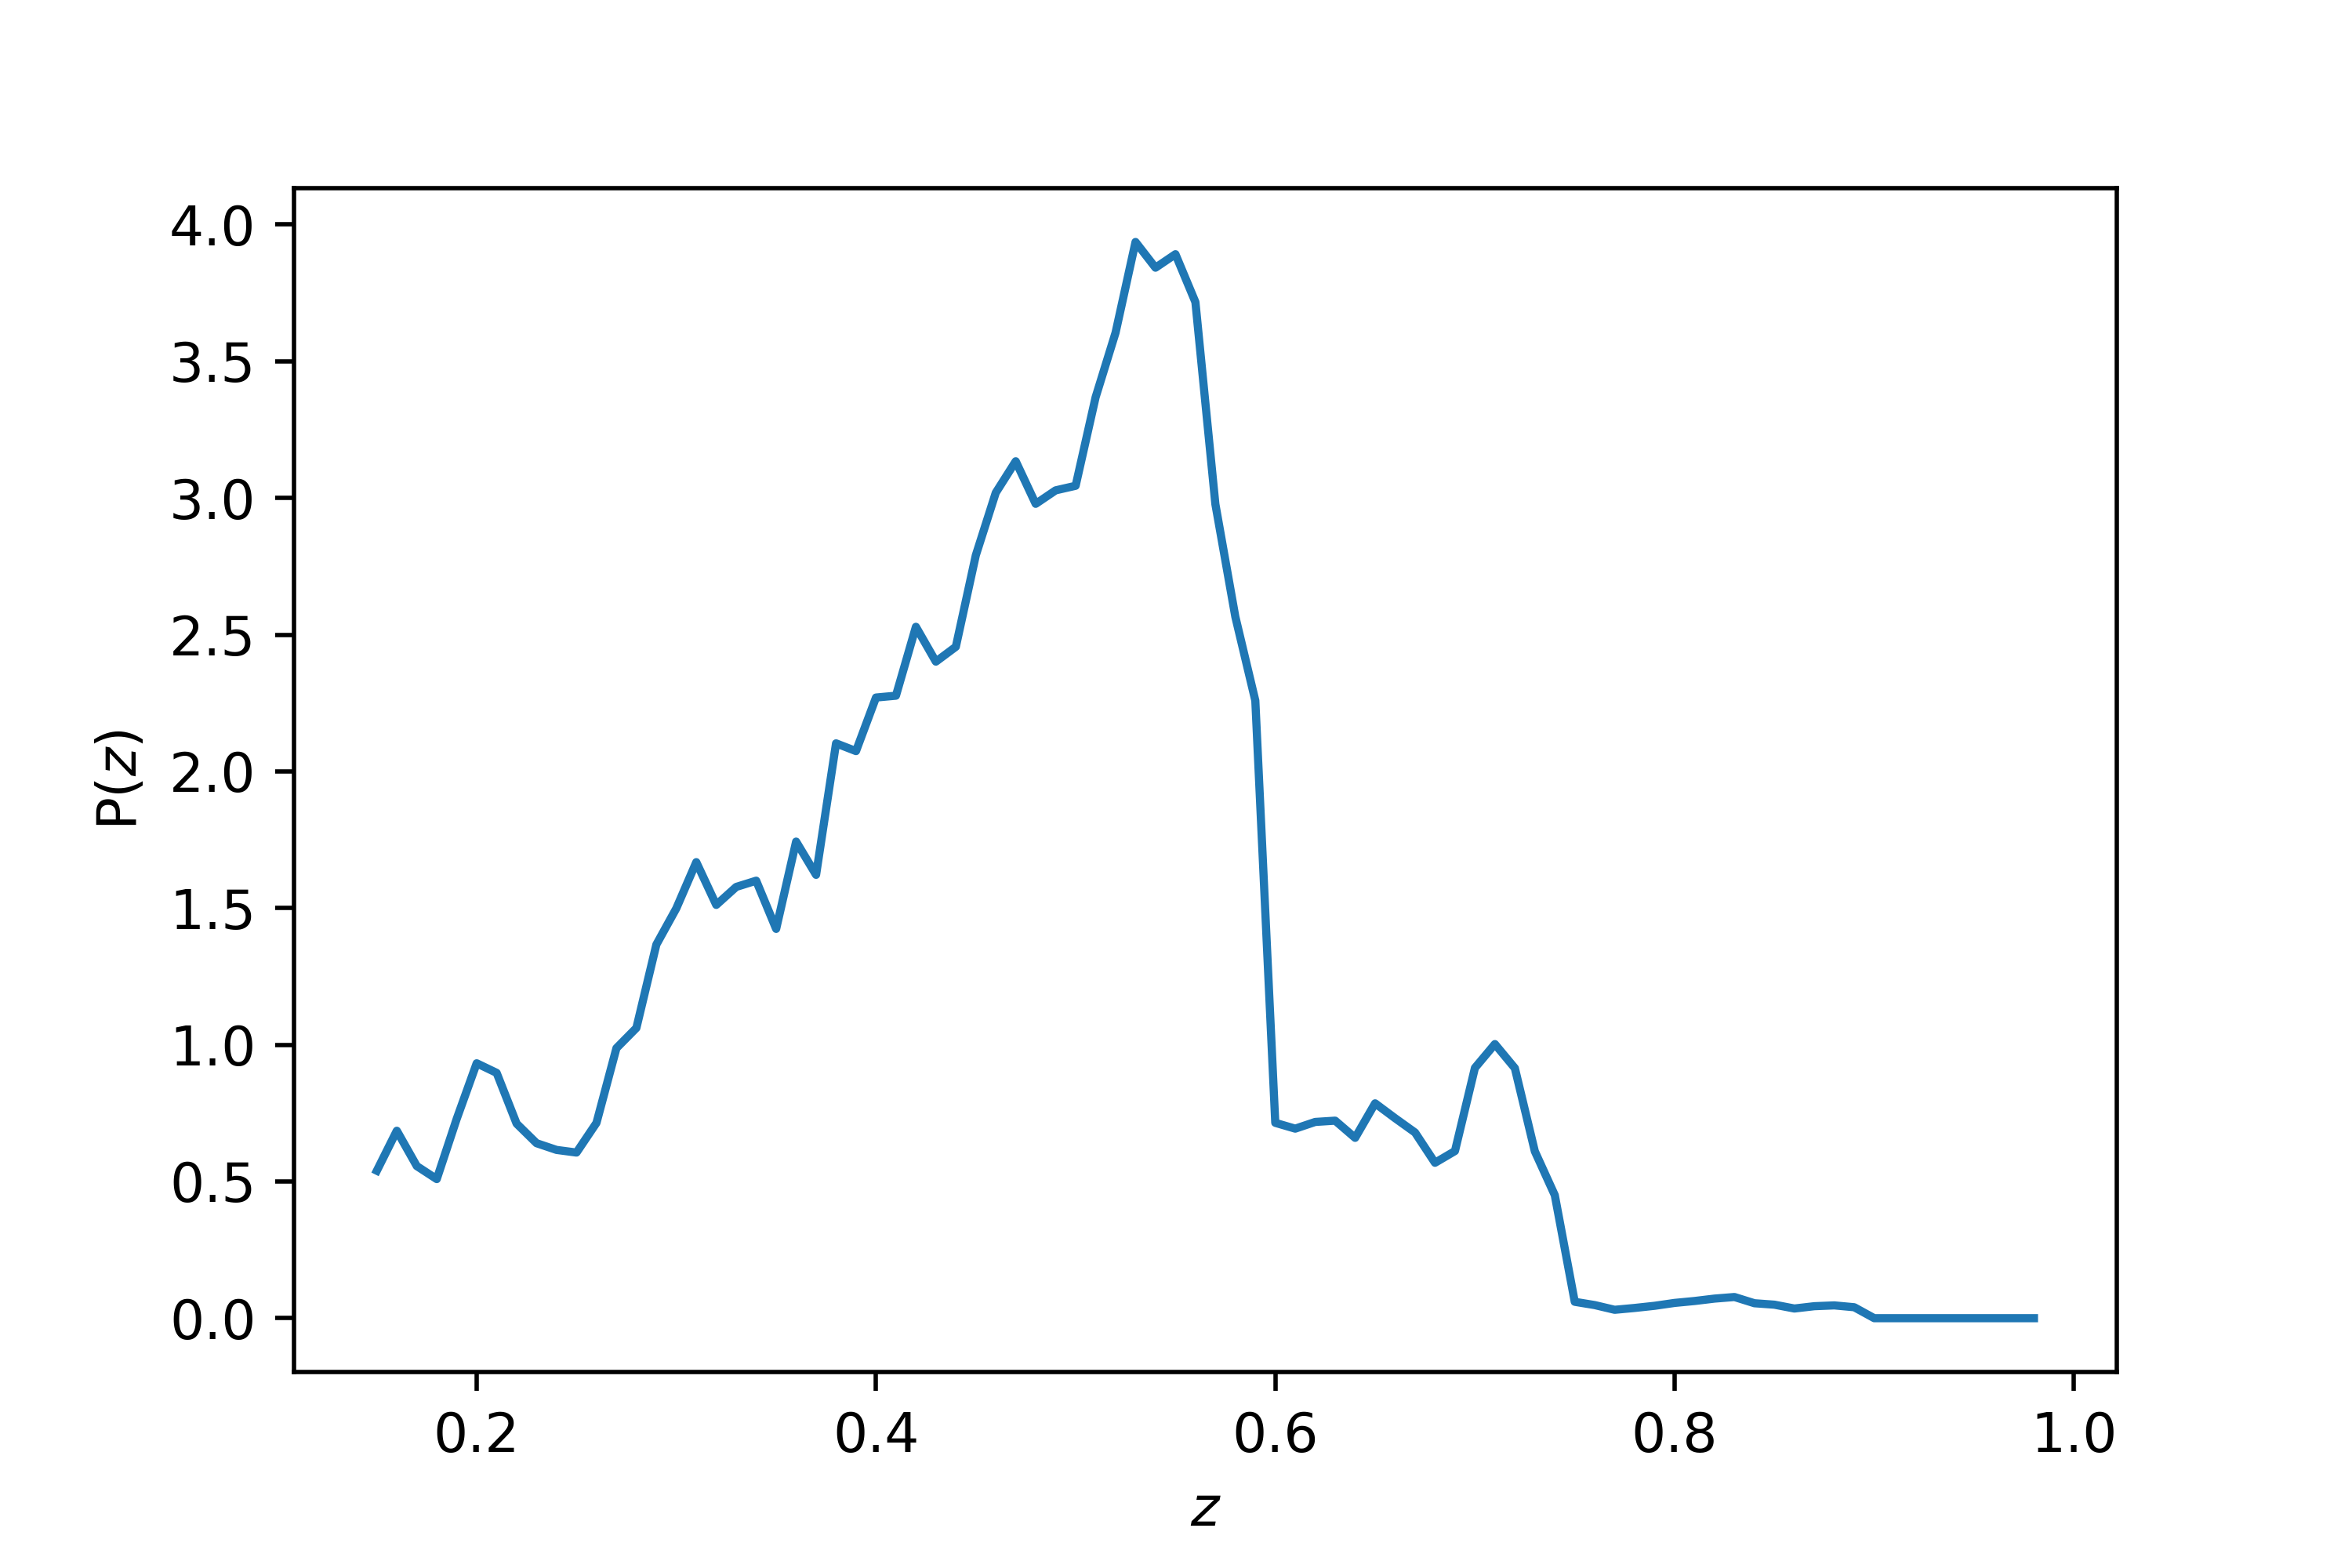
\includegraphics[scale=0.6]{/home/mitchell/Documents/masters/masters/thesis/Ver_2/figures/Redshift_Distribution.png}
\caption{Redshift Distributions of Physical Pairs. The pairs range from redshifts $z\approx0.15$ to $z\approx0.90$, with a mean redshift of $z\approx0.47$.}
\label{fig:physical:redshifts}
\end{figure}


\begin{figure}[h!]
\centering
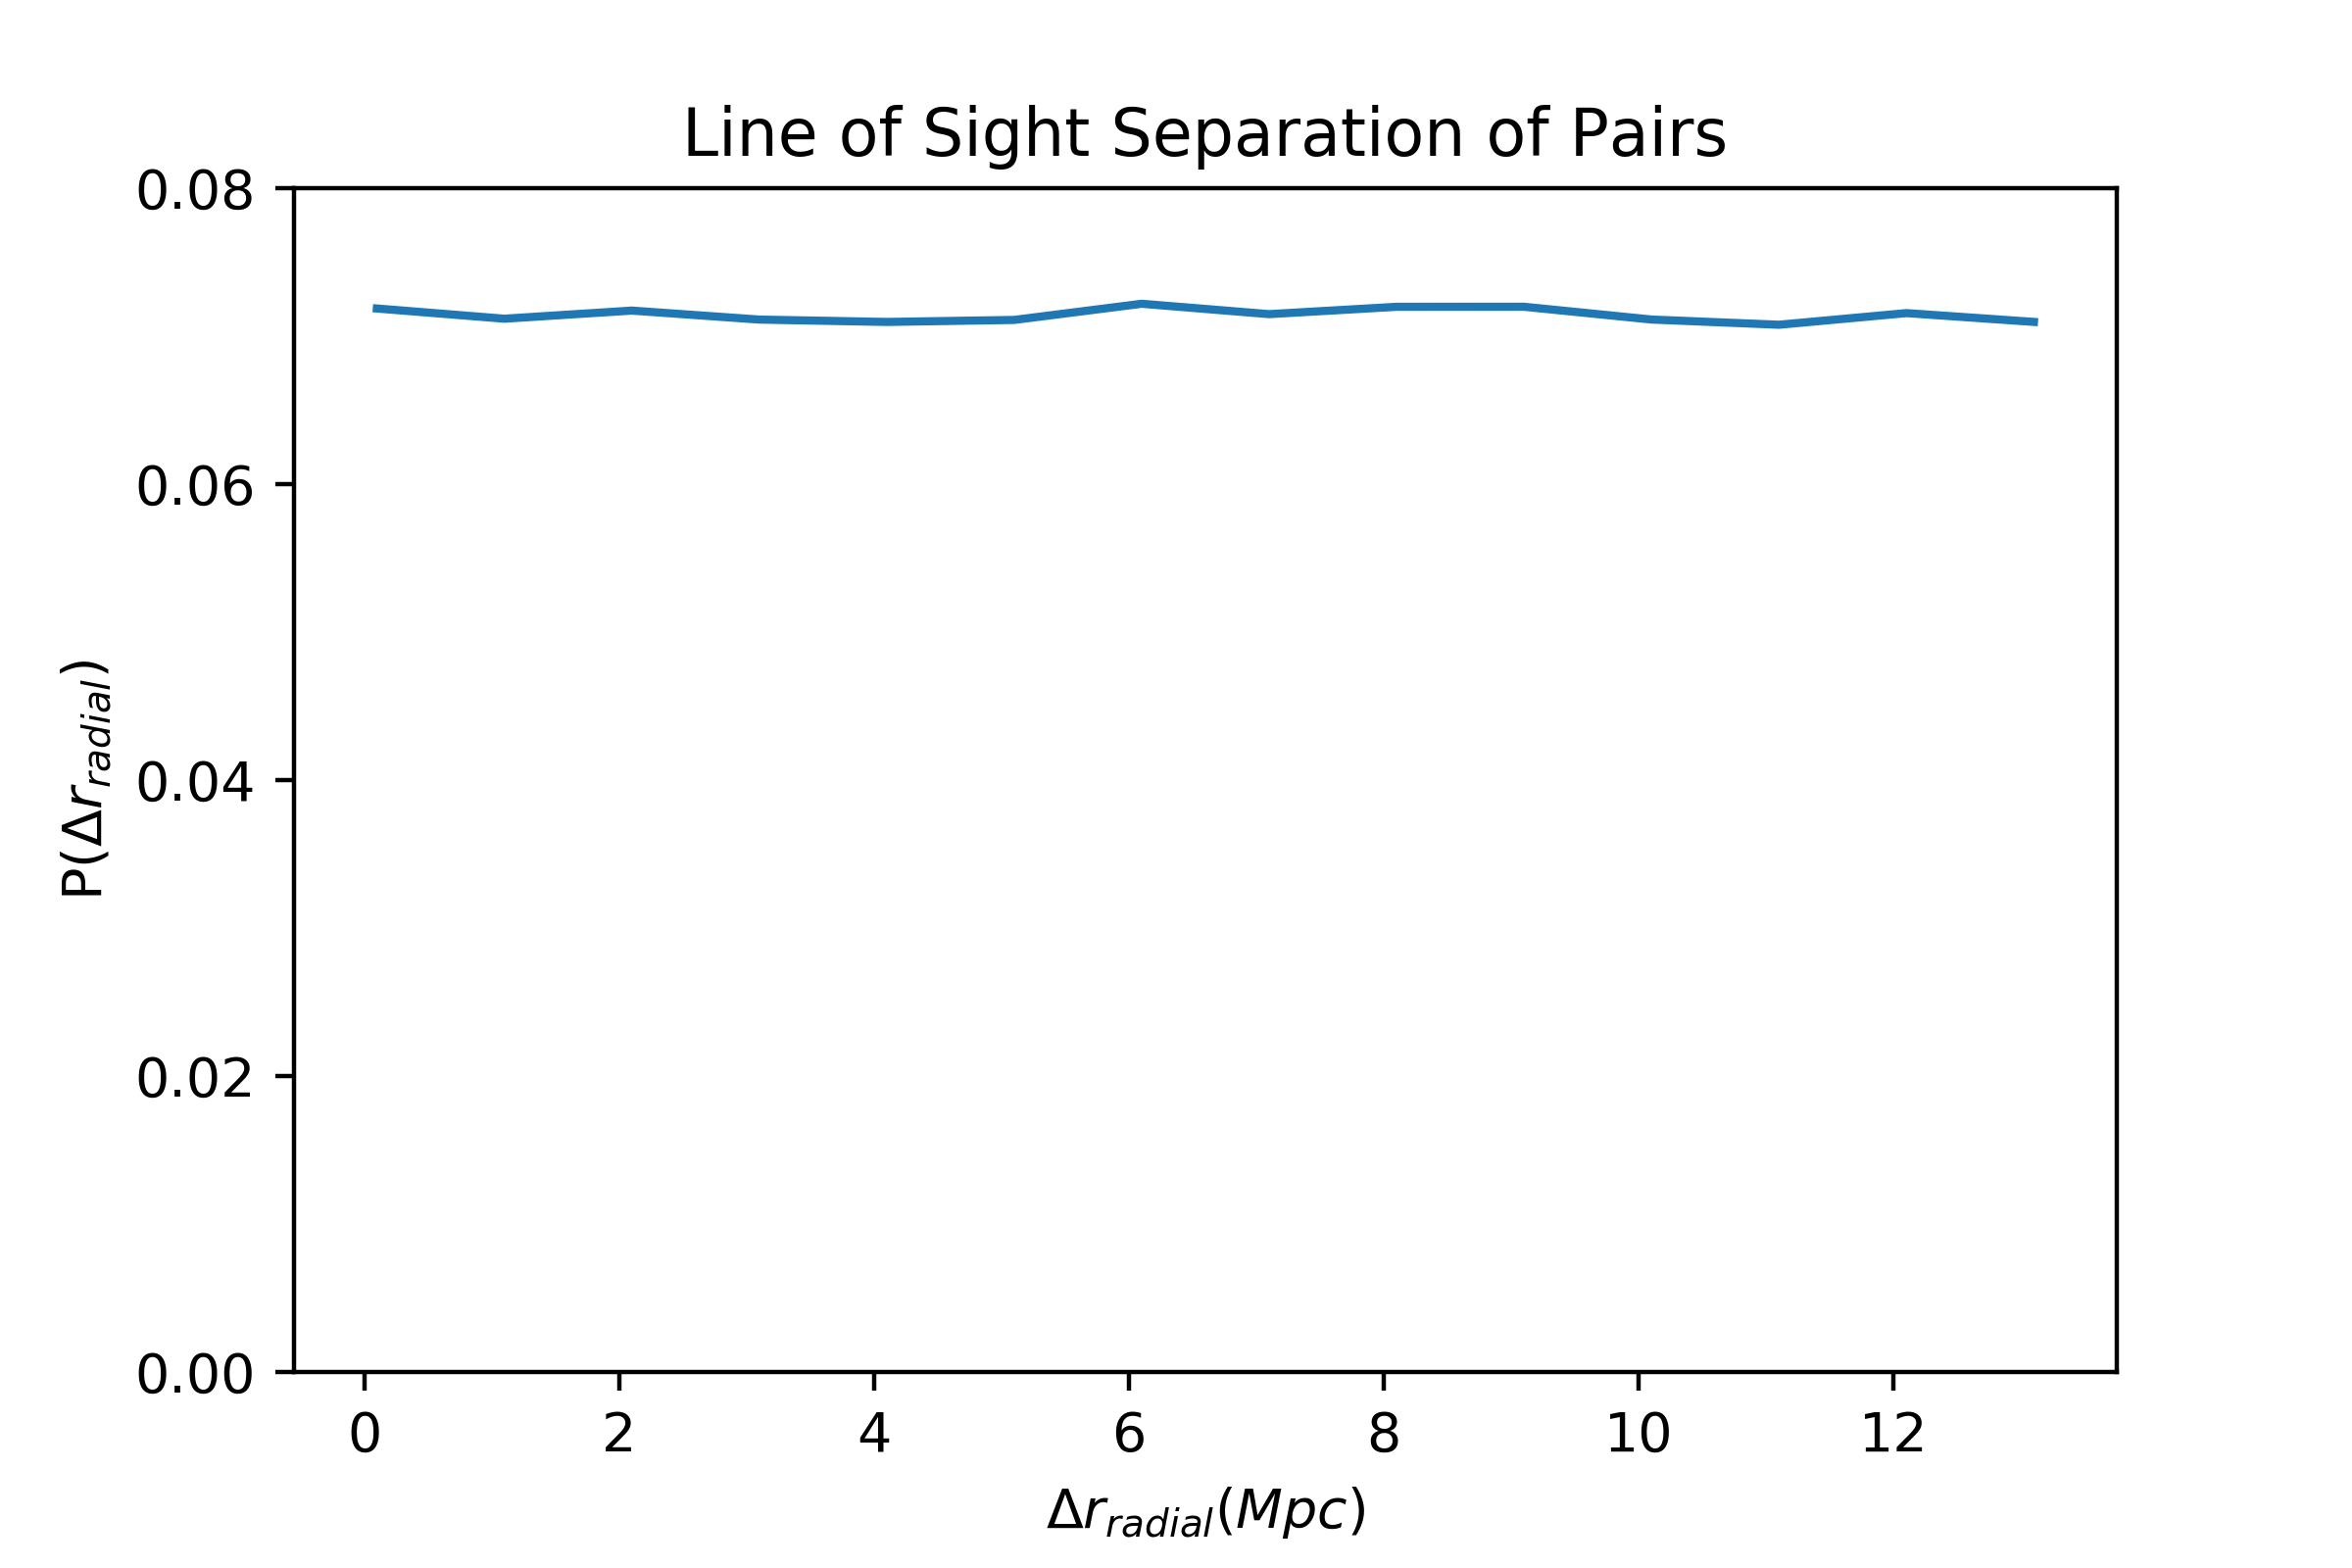
\includegraphics[scale=0.7]{/home/mitchell/Documents/masters/masters/thesis/Ver_2/figures/LOS_Separation.png}
\caption{Histogram of Line of Sight Separations of Galaxy Pairs. The distribution is relatively flat, with a minimum separation of $\SI{0}{\mega\parsec}$, and a maximum separation of $\SI{14.8}{\mega\parsec}$.}
\label{fig:physical:lineofsight}
\end{figure}



\begin{figure}[h!]
\centering
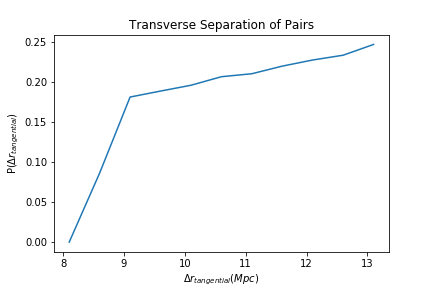
\includegraphics[scale=0.7]{/home/mitchell/Documents/masters/masters/thesis/Ver_2/figures/TRV_Separation.png}
\caption{Histogram of Transverse Separations of Unphysical Galaxy Pairs. The distribution is relatively flat, with a minimum seperation of $\SI{8.85}{\mega\parsec}$ and a maximum separation $\SI{20.7}{\mega\parsec}$. }
\label{fig:physical:transverse}
\end{figure}

The stacking procedure was performed on a Compton $y$ map produced from a combination of the South Pole Telescope SZ observing run, and the \emph{Planck} datasets. It made use of the $\SI{90}{\giga\hertz}$, $\SI{150}{\giga\hertz}$, and $\SI{2200}{\giga\hertz}$ from SPT-SZ, and the maps in the range of $\SI{100}{\giga\hertz}$ to $\SI{350}{\giga\hertz}$, as well as the $\SI{545}{\giga\hertz}$ map from \emph{Planck}, in the same manner as is described in \cite{2016ApJS..227...23C}. The algorithm for producing this map also took the half survey and half mission power spectra from \emph{Planck} as inputs. It minimised the contribution of the primary CMB, Cosmic Infrared Background (CIB), Instrumental, and Atmospheric sources as the primary sources of noise. The paper detailing the construction of this map is still under preparation by Lindsey Bleem. 

We performed the stack on a map with a resolution of $\SI{0.25}{\arcmin}$ per pixel, but the effective resolution, after combining the beam sizes of the various raw data maps, is closer to $\SI{2}{arcmin}$, so there is likely some interpolation in the output, which would have introduced a source of noise.


Stacking these pairs returns an average $y$ map, which is shown in figure \ref{fig:physical:stack}. The signal is dominated by the contribution of the galaxy halos, and so these will need to be effectively subtracted in order to evaluate the significance of the filament signal. To the eye, there appears to be some residual signal in between the two halos, which has not been driven to zero as a result of the stacking process. 


\begin{figure}[h!]
\centering
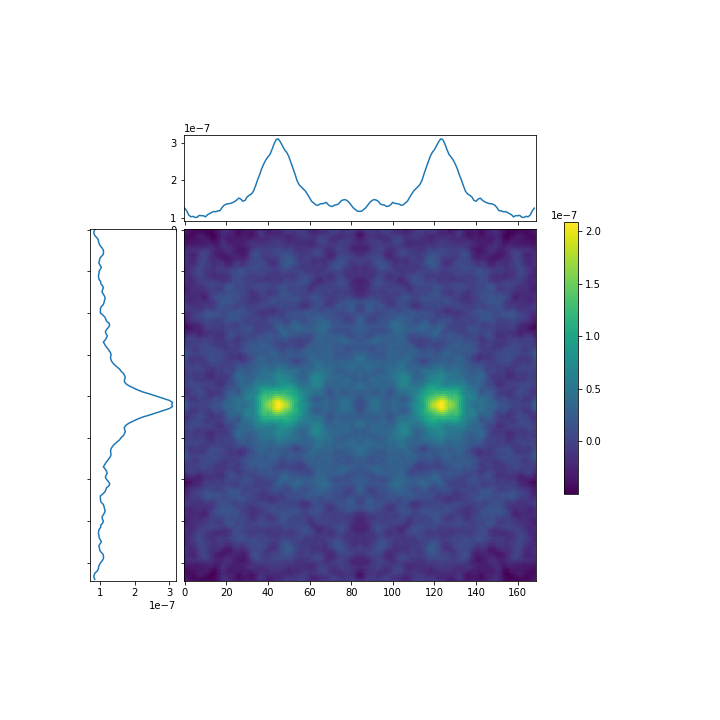
\includegraphics[scale=0.8]{/home/mitchell/Documents/masters/masters/thesis/Ver_2/figures/Stack.png}
\caption{Stacked Image of galaxy pairs. On the upper panel is the slice through the centre of the stack. The left panel displays a vertical slice through the left halo, which by the mirroring procedurce, will be effectively the same as the slice through the right halo.}
\label{fig:physical:stack}
\end{figure}


\section{Null Tests}
\subsection{Un-Physical Pairs}
We constructed a catalogue of unphysical pairs from the galaxies contained in both the SPTpol and DES survey footprints, with radial separations between $\SI{100}{\per\h\mega\parsec}$ and $\SI{200}{\per\h\mega\parsec}$, and transverse separations between $\SI{6}{\per\h\mega\parsec}$ and $\SI{14}{\per\h\mega\parsec}$. 

\begin{figure}[h!]
\centering
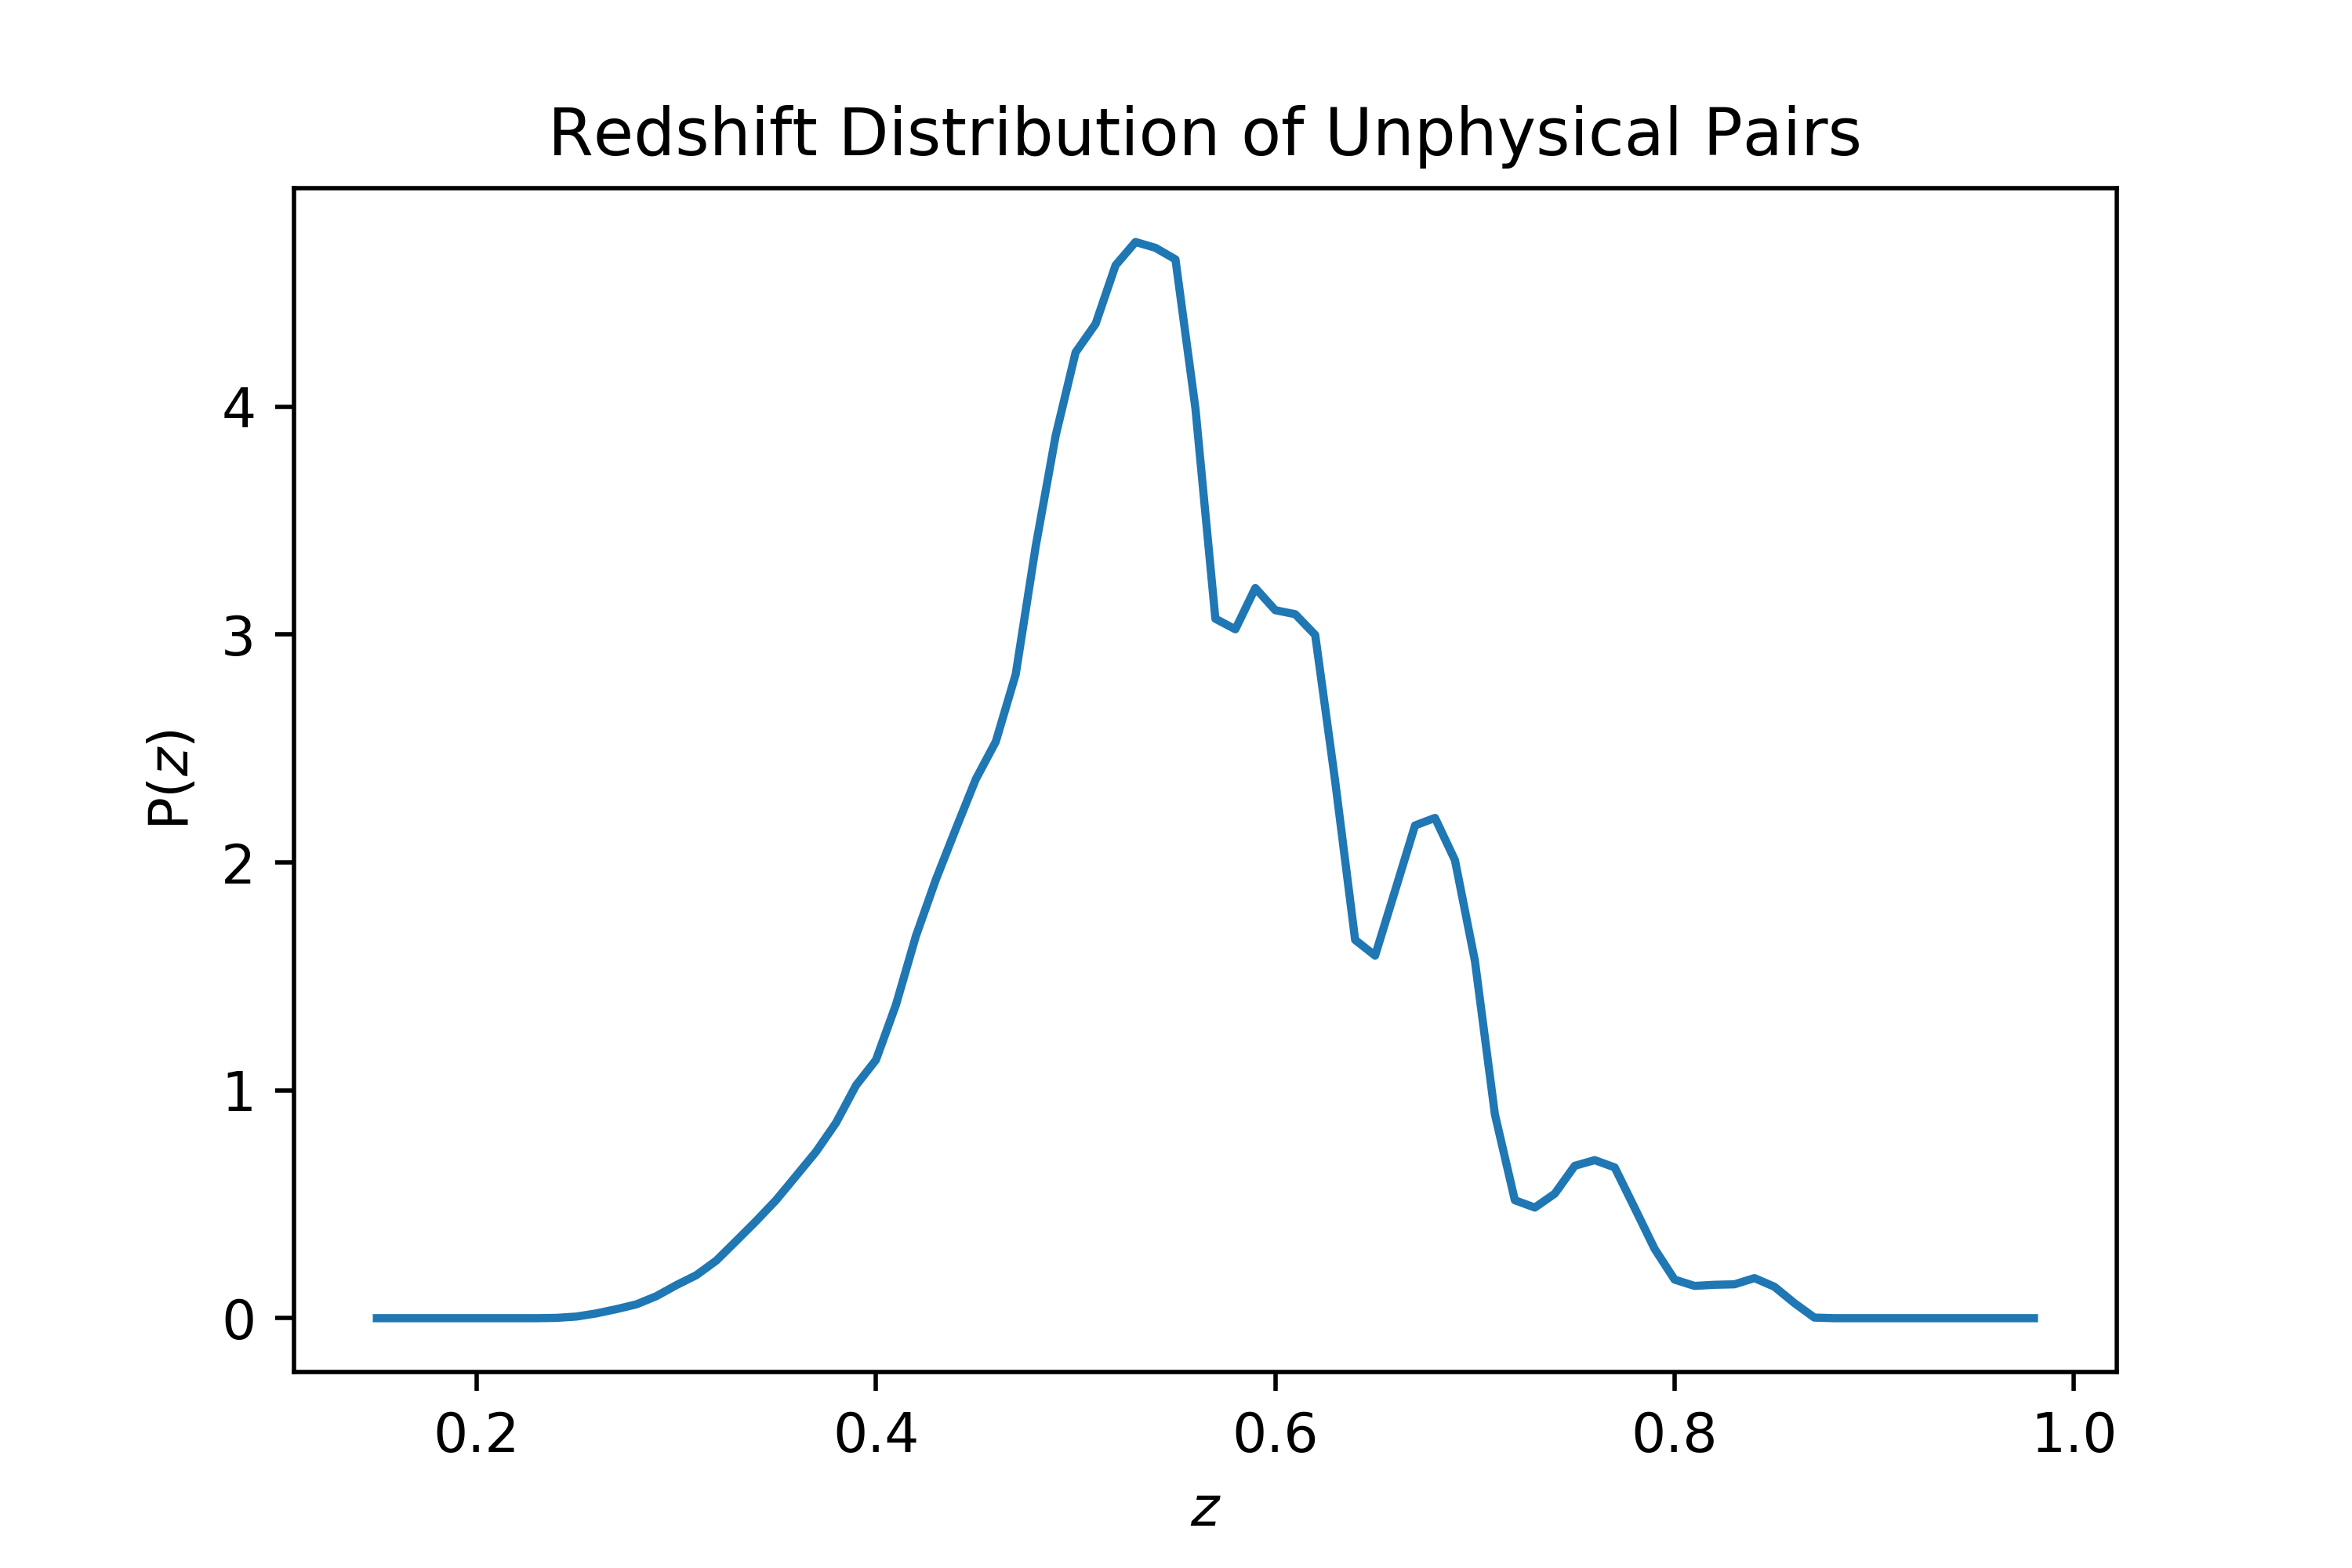
\includegraphics[scale=0.7]{/home/mitchell/Documents/masters/masters/thesis/Ver_2/figures/UnPhysical_Redshift_Distribution.png}
\caption{Redshift Distributions of Unphysical Pairs. The pairs range from redshifts $z\approx0.24$ to $z\approx0.87$, with a mean redshift of $z\approx0.55$. When compared to the physical pairs, this set has a higher mean redshift, and more pairs in higher redshift bins.   }
\label{fig:unphysical:redshifts}
\end{figure}
As can be seen in \ref{fig:unphysical:redshifts}, the distribution of redshifts is generally skewed towards higher redshifts than for the physical pairs. This is likely due to the inherent errors assosciated with the photometric redshifts in the DES redMaGiC survey. Lower redshifts are more likely to be more precise, since the photometric errors for redshift are given by $\Delta z= 0.01(1+z)$, and so be exculded by the line of sight cuts. The other effect which may influence this is the fact that there are far more pairs in the unphysical dataset than in the physical dataset. 


This produced a set of unphysical pairs containing $\sim 670000$ pairs, with a mean line of sigh separation of $\SI{220}{\mega\parsec}$, and a mean transverse separation of $\SI{12.5}{\mega\parsec}$.


\begin{figure}[h!]
\centering
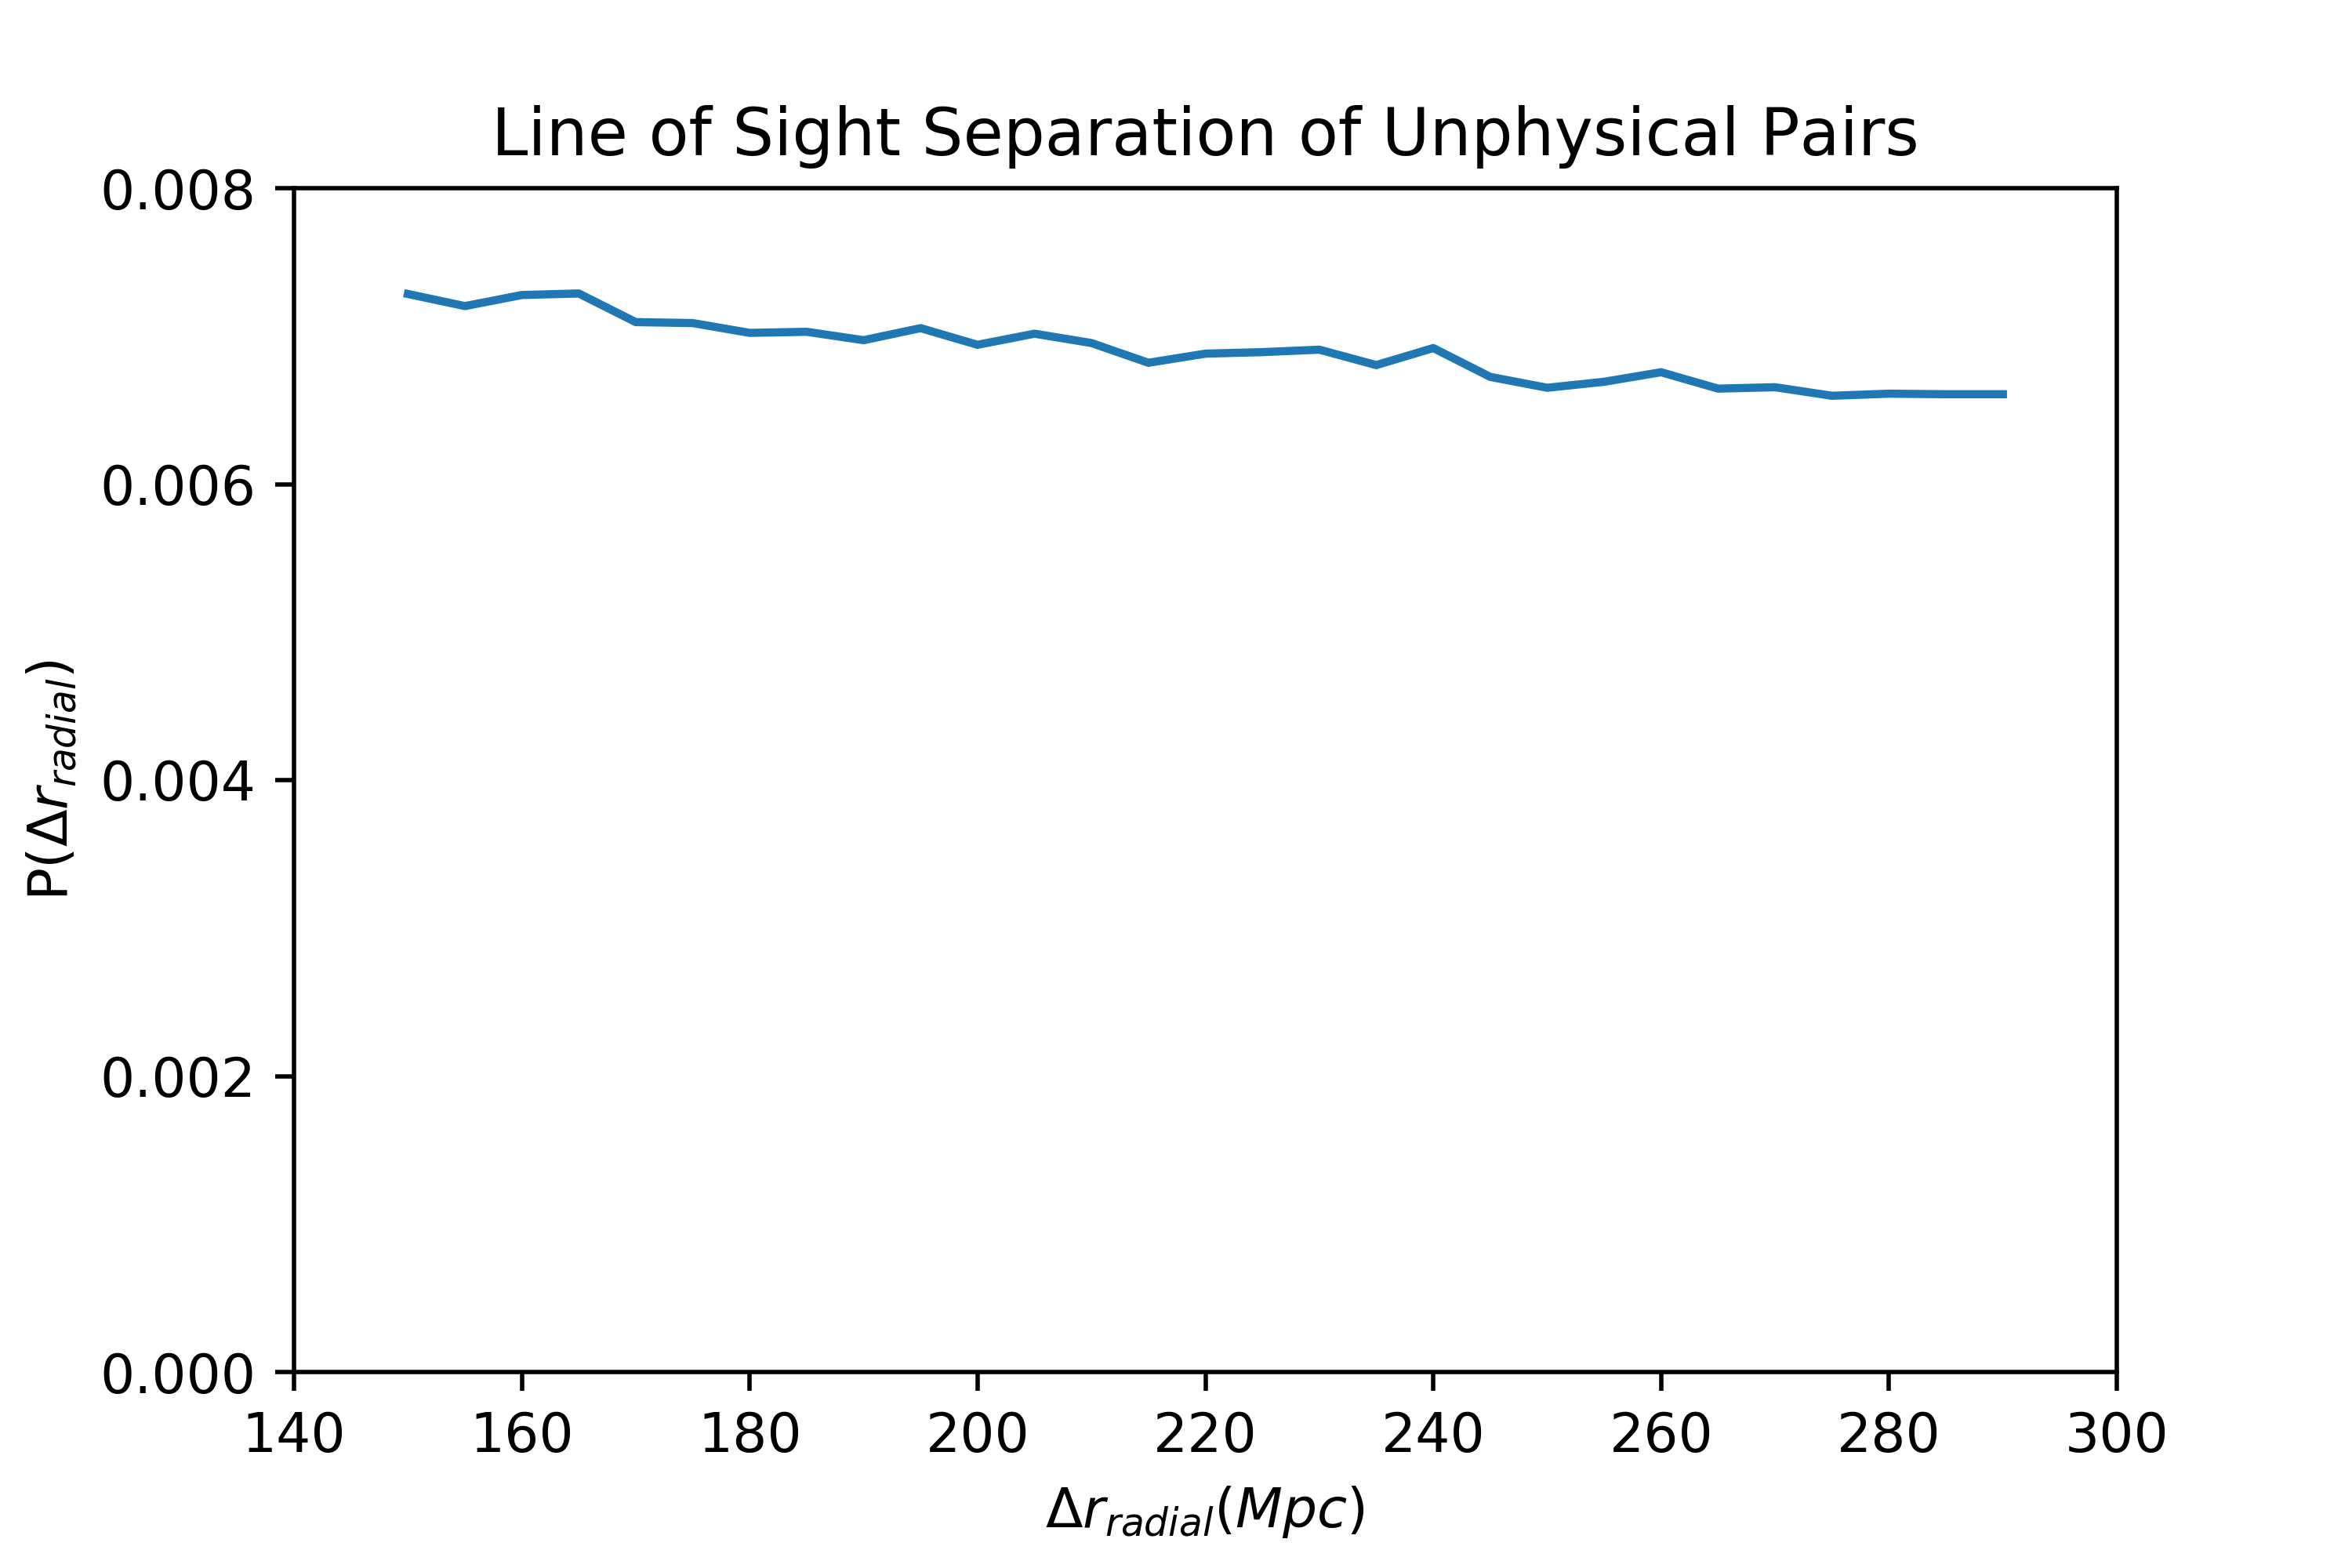
\includegraphics[scale=0.7]{/home/mitchell/Documents/masters/masters/thesis/Ver_2/figures/UP_LOS_Separation.png}
\caption{Histogram of Line of Sight Separations of Unphysical Galaxy Pairs. The distribution is relatively flat, with the same shape as the physical pairs, a minimum separation of $\SI{147}{\mega\parsec}$, and a maximum separation of $\SI{295}{\mega\parsec}$.  }
\label{fig:unphysical:lineofsight}
\end{figure}

The choice was made to consider unphysical pairs with a line of sight separation in excess of $\SI{100}{\per\h\mega\parsec}$ because at large redshifts, the errors assosciated with the photometric redshifts can place a very large range on the possible distance to a given galaxy, and we want to be very careful to exclude galaxy pairs that might have a connecting filament between them. 

\begin{figure}[h!]
\centering
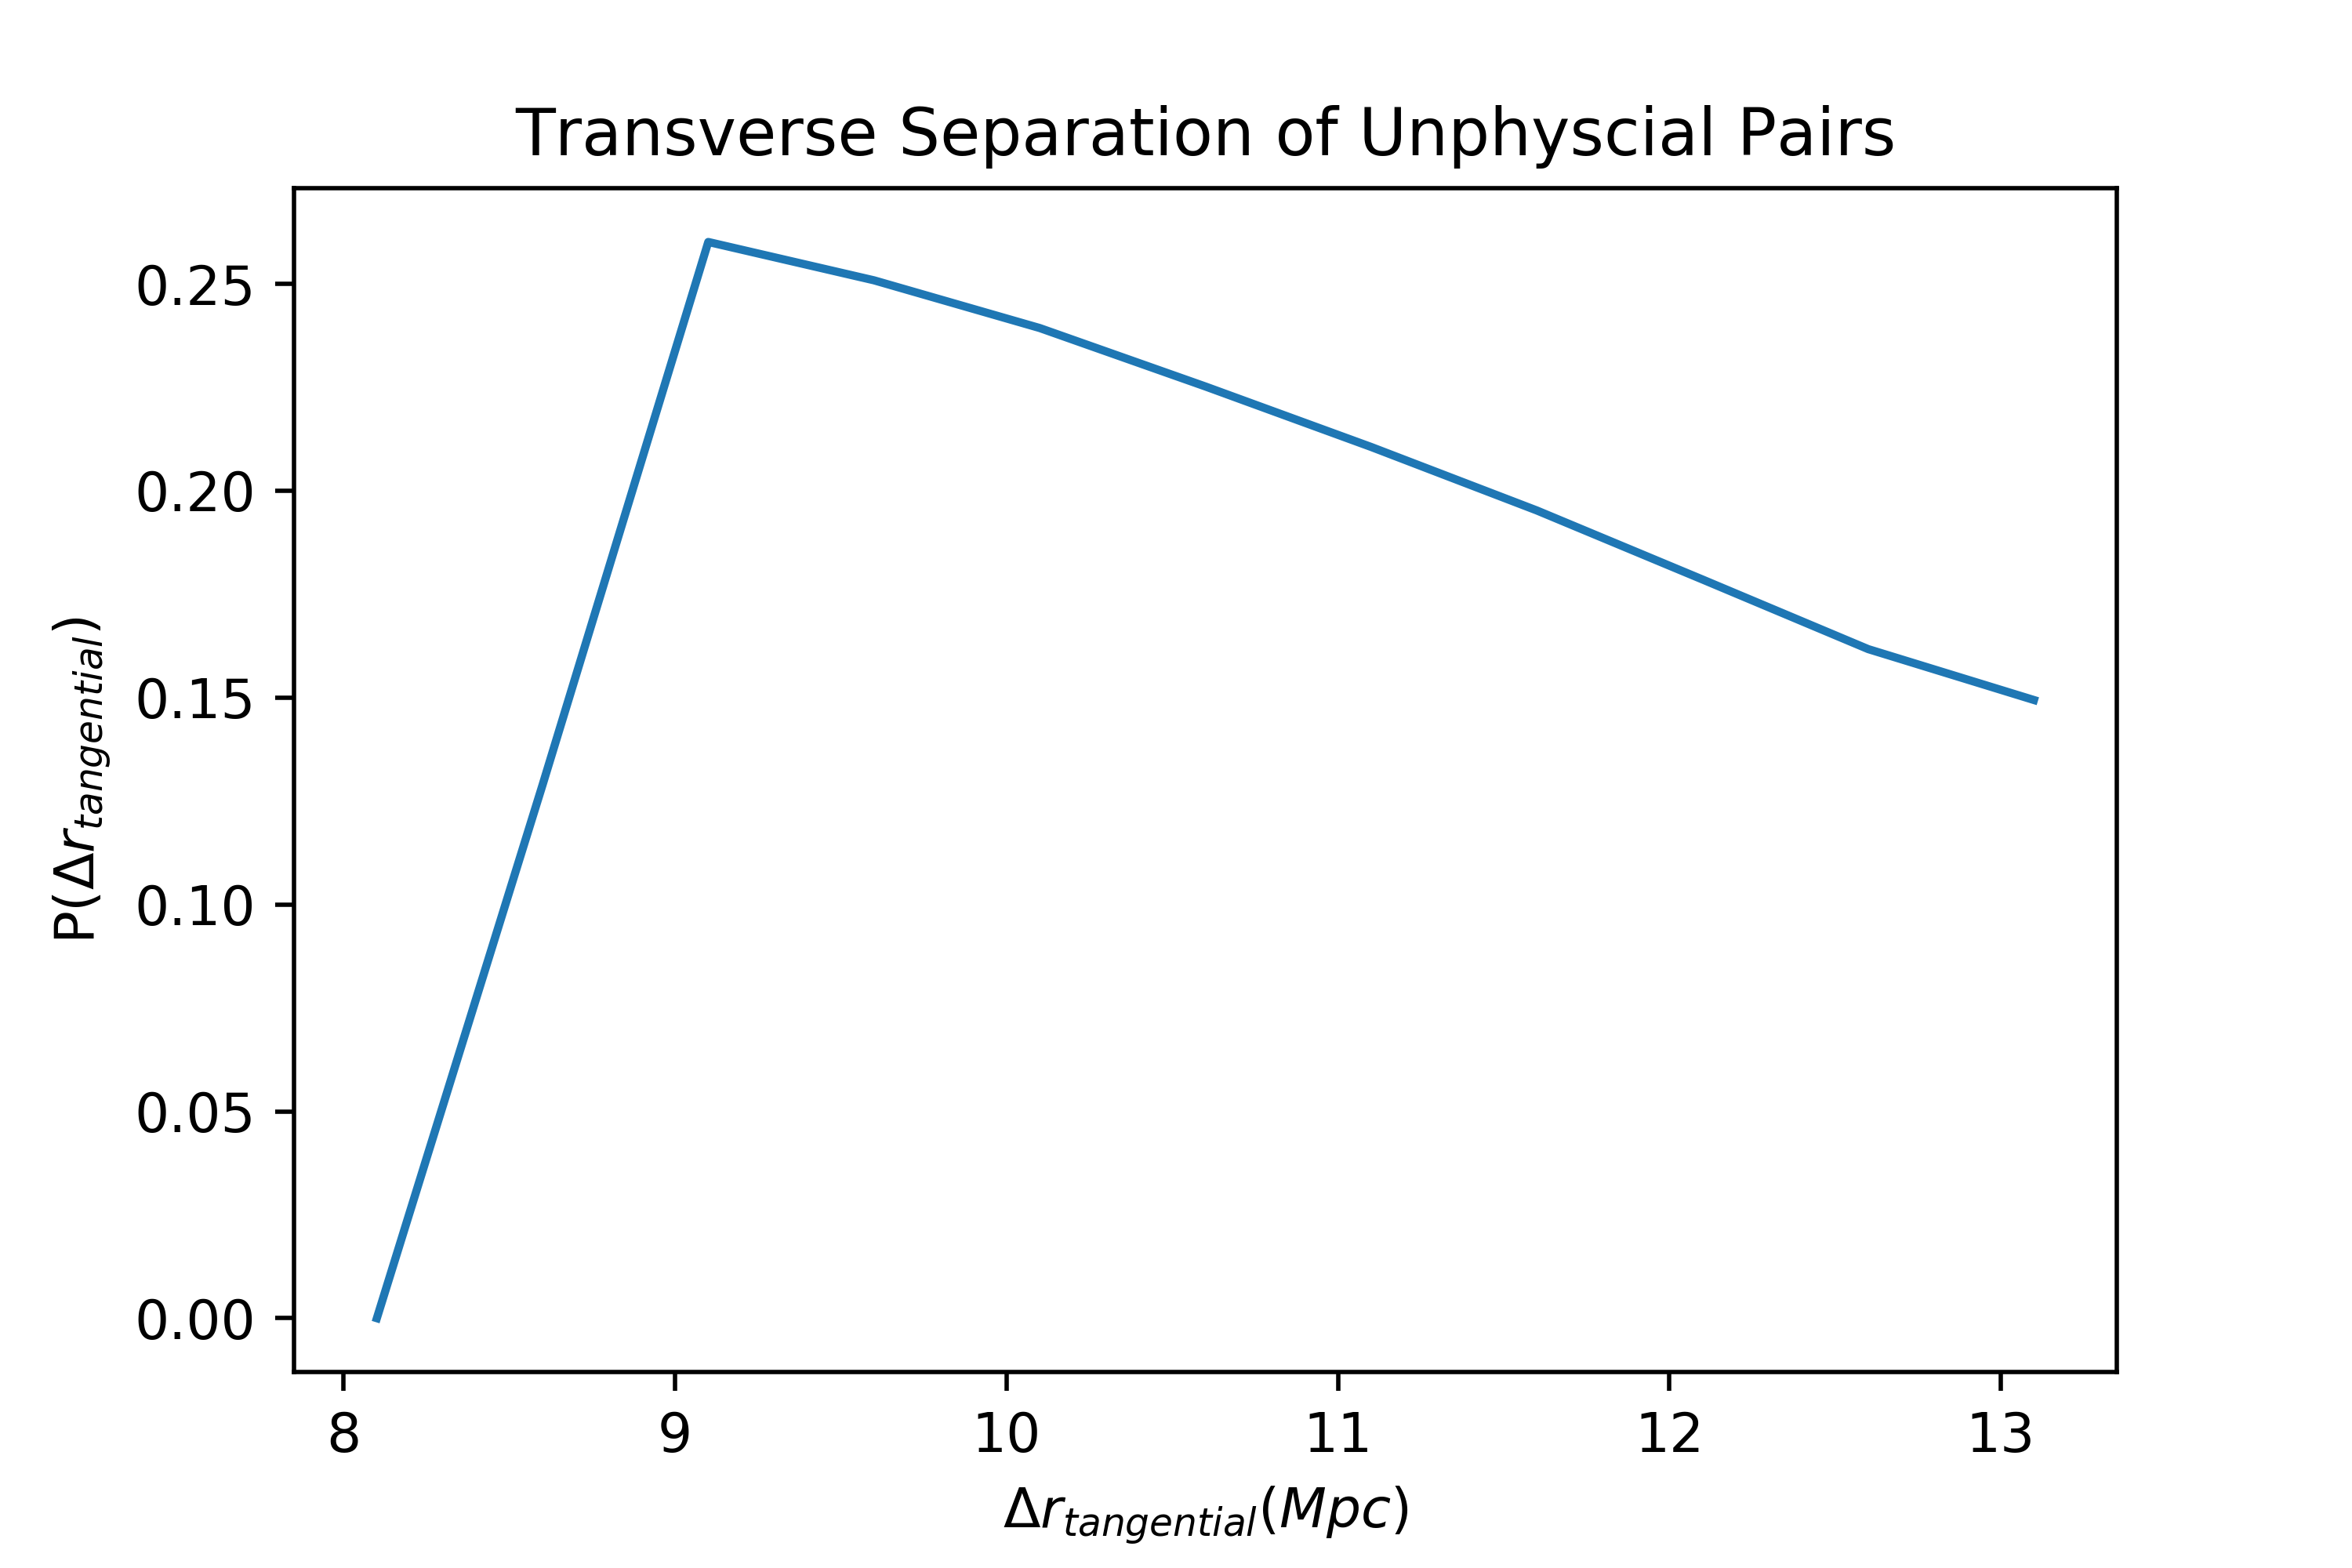
\includegraphics[scale=0.7]{/home/mitchell/Documents/masters/masters/thesis/Ver_2/figures/UP_TRV_Separation.png}
\caption{Histogram of Transverse Separations of Unphysical Galaxy Pairs. The distribution is relatively flat, with a minimum seperation of $\SI{8.85}{\mega\parsec}$ and a maximum separation $\SI{20.7}{\mega\parsec}$. This has the same overall shape as the physical pairs data set, except the relative population in the higher separation bins decreases, rather than increases.}
\label{fig:unphysical:transverse}
\end{figure}

Performing the stacking procedure on the unphysical dataset gives the stack shown in figure \ref{fig:unphysical:stack}. To the eye, in both the 2D slice and the 3D colour map, it appears that there is less filamentary signal than for the physical pairs. 

\begin{figure}[h!]
\centering
\includegraphics[scale=0.6]{/home/mitchell/Documents/masters/masters/thesis/Ver_2/figures/UnPhysical_Stack.png}
\caption{Stacked Image of Unphyiscal pairs.}
\label{fig:unphysical:stack}
\end{figure}

If we fit the two halos for gaussian profiles (shown in figure \ref{fig:unphysical:fit}) , along with some constant offset, we can see very clearly that there appears to be no residual signal left. The mean of this residual is $3.48 \times 10^{-18}$, with a variance of $1.13 \times 10^{-16}$, effectively making this noise. 


\begin{figure}[h!]
\centering
\includegraphics[scale=0.6]{/home/mitchell/Documents/masters/masters/thesis/Ver_2/figures/unphysical_halo_fit.png}
\caption{Gaussian Fit to Unphysical Pairs}
\label{fig:unphysical:fit}
\end{figure}

\subsection{Random Stack}

Performing a stack on a set of pseudo-randomly selected slices of the CMB, with the same galactic latitude as the physical pairs, we produced a stack like the one shown in \ref{fig:random:stack}. This has no discernable structure, except for the small circular signal in the centre of the map. This is likely due to the rescaling effect still rescaling the CMB as if it were trying to align pairs. Because the angle that the pairs need to be rotated by should be evenly distributed, there should be some level of correlation in the stack.

\begin{figure}[h!]
\centering
\includegraphics[scale=0.6]{/home/mitchell/Documents/masters/masters/thesis/Ver_2/figures/Rand_Pos_Stack.png}
\caption{Stack of pseudo-random slices}
\label{fig:random:stack}
\end{figure}